\section{Algorithm}%
\label{Algorithm}

Alice and Bob each has a set of devices containing their files, \eg a 
smartphone, laptop and a desktop computer.
Alice and Bob meet in a café carrying only their smartphones and Alice wants to 
share a file, \(f\), with Bob.
Alice's smartphone knows some metadata of \(f\) and that it resides on Alice's 
desktop computer.
She gives some metadata about \(f\) to Bob, at least the file size.
Bob creates an onion route of low-availability devices with some subset of Bob's 
devices as the destination.
The layers of the route are chosen such that the probability of all devices 
being offline at the same time is low.
Bob gives this route to Alice.
Alice's smartphone ensures that her desktop computer (containing the file \(f\)) 
gets the route and the instruction to send \(f\) using this route.
When Alice's desktop computer receives this instruction it will create the first 
half of the route and concatenate it with Bob's route, then transfer \(f\) to 
Bob.
In this section we will present the details of the necessary algorithms.

We have a set of users, \(U\), each user \(u\in U\) has a set of devices, 
\(D_u\).
We call \(D_u\) the device swarm of \(u\).
Alice, \(a\in U\), has a device swarm, \(D_a\), and Bob, \(b\in U\) has a device 
swarm, \(D_b\).
We let \(D = \cup_{u\in U} D_u\) be the set of all devices, the global device 
swarm.
Without loss of generality, we will use Alice, with device swarm \(D_a\), and 
Bob, with device swarm \(D_b\), as examples.

\subsection{Alice's device swarm}%
\label{local-swarm}

Each of Alice's (and Bob's) devices will keep track of its own online and 
offline behaviour.
They will use a protocol like Sprinkler~\cite{luxey:hal-01704172} to learn about 
each other's online--offline behaviour.
\commentDaniel{Is that correct?}
This allows Alice's device swarm to infer a behavioural model for the device 
swarm and do internal scheduling based on the probability of being online.

\subsubsection{Sharing the user's behavior}% (fold)
\label{ssub:sharing_the_user_s_behavior}

Each device initially only knows when it is connected. 
To make a model of the user's behavior, they need to know the whole observation sequence $O$: which device is online at each time step.
To do so, they employ a probabilistic dissemination protocol, 
\textsc{Sprinkler}~\cite{luxey:hal-01704172}.
This allows devices to gossip any new connection information to random peers in 
the local swarm, ensuring that all devices know the full observation sequence 
with a very high probability.
\textsc{Sprinkler} has shown resilient to device churn~\cite{luxey:cascade}, and 
is thus perfectly suited for our purpose, where a user's devices often 
disconnect and reconnect. 

\commentAL{Then we \textbf{maybe} do predictions as \textbf{maybe} shown in 
  \cref{sec:user_model}.}


% subsubsection sharing_the_user_s_behavior (end)

\subsubsection{Sharing files location}% (fold)
\label{ssub:sharing_files_location}

We do stuff and things work.

% subsubsection sharing_files_location (end)


\subsection{The global device swarm and random peer sampling}

\commentDaniel{%
  We must cover how to do \(\Pr[d \text{ offline at time } t]\) as used in 
  \cref{ExtendRoute}.
  This is probably part of getting random peers in the same place.%
}

\commentDaniel{%
  What is the probability distribution of the peer sample that we get?
  Will it be close to uniformly random?%
}

\NewAlgorithm{\GetRandomPeer}{GetRandomPeer}

Every time a device is online, it participates in the random peer sampling 
protocol.
If a device is sampled it provides the following information:
\begin{itemize}
  \item its address, \(d\);
  \item its public key, \(\pk_d\);
  \item the probability of being online, \(p_d\).
\end{itemize}
We will denote this by the following algorithm \((d, \pk_d, p_d)\gets 
  \GetRandomPeer\), which will be used below.
The probability of being online, \(p_d\), is inferred as above 
(\cref{local-swarm}).


\NewScheme{\SPOR}{SPOR}

\subsection{\(\SPOR\): Stateless Predictive Onion Routing}%
\label{SPOR}

\NewAlgorithm{\Send}{Send}
\NewAlgorithm{\Fwd}{Forward}
\NewAlgorithm{\Recv}{Receive}
\NewVariable{\rdv}{rdv}

We have the Stateless Predictive Onion Routing scheme, \SPOR, which provides 
probabilistically onion-routed message passing.
Instead of providing only one address per hop in the route (as in \eg 
Tor~\cite{Tor}), \(\SPOR\) provides several alternatives for the next hop 
depending on their probability of being online.
To do this, \(\SPOR\) provides stateless algorithms for the onion-routing.

\(\SPOR\) provides three algorithms: \(\SPOR[\Send]\) (\cref{SPORSend}), 
\(\SPOR[\Fwd]\) (\cref{SPORFwd}) and \(\SPOR[\Recv]\) (\cref{SPORRecv}).
Say Alice wants to send a message \(m\) to Bob.
Bob uses \(\SPOR[\Recv]\) to create a probabilistic onion route \(H_\rdv\) from 
a rendez-vous point to his own device swarm --- all the hops on the route are 
chosen by Bob uniformly at random.
Bob gives \(H_\rdv\) to Alice using an out-of-band channel, \eg using his phone.
Alice uses \(\SPOR[\Send]\) at some later time to send the message to Bob using 
any of her devices.
\(\SPOR[\Send]\) extends the route \(H_\rdv\) with some hops of Alice's choosing 
(uniformly randomly chosen), then starts to forward the message (using 
\(\SPOR[\Fwd]\)) through the hops on the route to Bob.
This process is illustrated in \cref{fig:file-exchange}.

\begin{figure}
  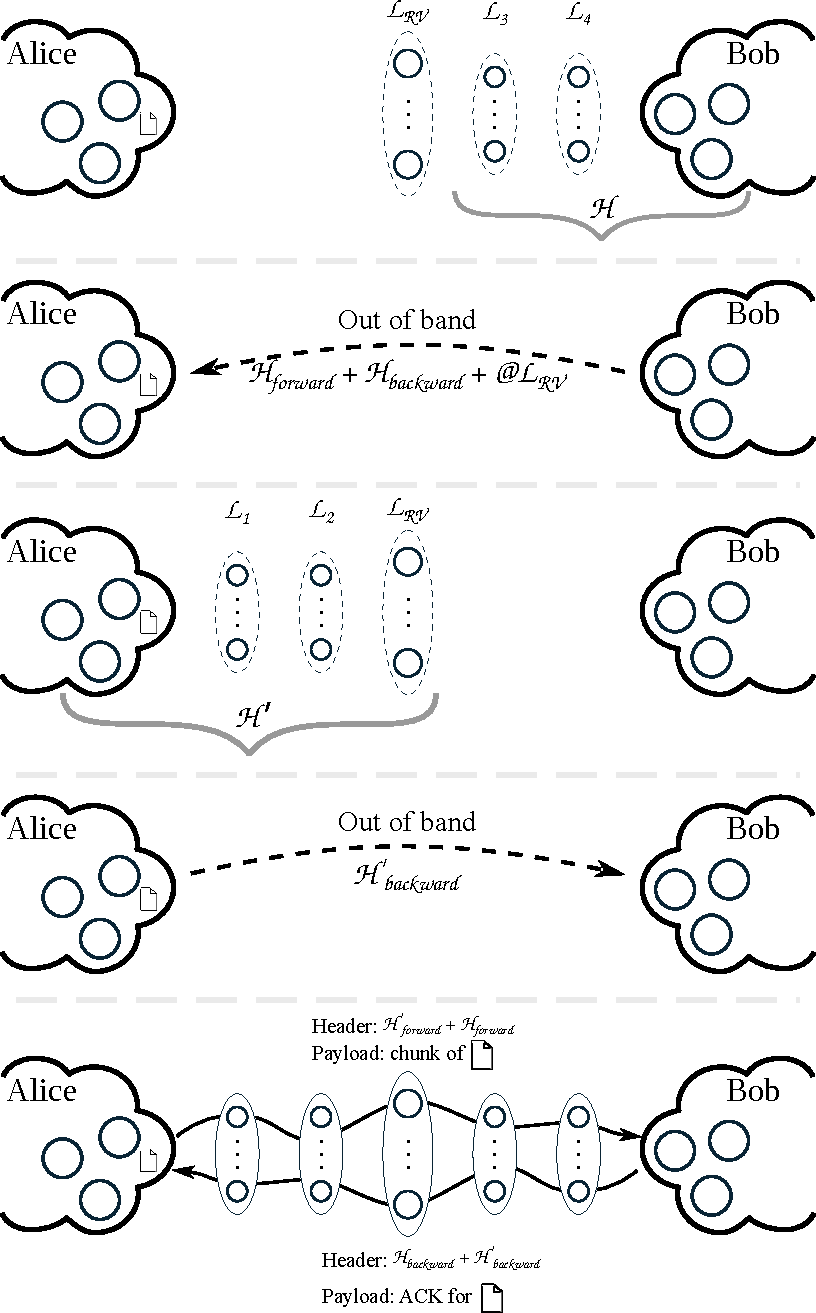
\includegraphics[width=\linewidth]{figures/file_exchange.pdf}
  \caption{\label{fig:file-exchange}%
    A schematic of Alice and Bob sending a message using \(\SPOR\).
  }
\end{figure}

\NewAlgorithm{\ExtendRoute}{ExtendRoute}
\NewAlgorithm{\CreateOnionLayer}{CreateOnionLayer}

\begin{figure}
  \begin{algorithmic}
    \Require{%
      $H$ is a header of the form \(D\concat H'\) or \(D\concat \top\), where 
      \(D\) is a set of device addresses.
      $\pk_D$ is the public key of device set $D$.
      $L$ is the length of the route,
      $\theta$ is the threshold of probability of failure.%
    }
    \Function{\ExtendRoute}{$H, L, \theta$}
      \If{$L\leq 0$}
        \State \Return $H$
      \EndIf
      \State $D\gets \CreateOnionLayer[\theta]$
      \State $H\gets D\concat \DeBEenc[\mpk, D, H]$
      \State \Return $\ExtendRoute[H, L-1, \theta]$
    \EndFunction

    \Function{\CreateOnionLayer}{$\theta$}
      \State $(d, \pk_d, p_d)\gets \GetRandomPeer$
      \Comment We use \(d\) as shorthand for this tuple.
      \State $D\gets \{d\}$
      \While{$\prod_{d\in D} p_d > \theta$}
        \State $d\gets \GetRandomPeer$
        \State $D\gets D\cup \{d\}$
      \EndWhile
      \State \Return $D$
    \EndFunction
  \end{algorithmic}
  \caption{\label{ExtendRoute}%
    The \(\ExtendRoute\) algorithm extends a route \(H\) with \(L\) hops and 
    failure threshold of \(\theta\) for each hop in the route.
    Thus the probability of failure for the extension is \(1 - (1 - \theta)^L\).
    The function \(\GetRandomPeer\) is any random peer-sampling algorithm.
  }
\end{figure}

\NewAlgorithm{\Store}{Store}
\NewAlgorithm{\Dec}{Dec}
\NewVariable{\sk}{sk}

\begin{figure}
  \begin{algorithmic}
    \Require{%
      $D$ is the set of alternative recipient devices.
    }
    \Function{\SPOR[\Recv]}{$D$}
      \State $H_\rdv\gets \ExtendRoute[D\concat \top, L, \theta]$
      \State \Return $H_\rdv$
        \Comment{Give to sender out-of-bound.}
    \EndFunction

    \Function{\Store}{$m$}
      \State $m\gets \DeBEdec[\mpk, \sk, c_m]$
      \If{$m = \bot$}
        \State \Return $\bot$
      \EndIf
      \State Store $m$ to disk.
      \State \Return $\top$
    \EndFunction
  \end{algorithmic}
  \caption{\label{SPORRecv}%
    The \(\SPOR[\Recv]\) algorithm prepares the recipient for receiving a file.
    It creates a probabilistic onion-route from a rendez-vous point to its own 
    devices and returns the route to the sender.
    The \(\Store\) algorithm is used by the local \(\SPOR[\Fwd]\) algorithm to 
    store messages intended for itself.
  }
\end{figure}

\begin{figure}
  \begin{algorithmic}
    \Require{%
      $m$ is the message to be sent,
      $H_\rdv$ is the onion-route given by the recipient.
    }
    \Function{\SPOR[\Send]}{$H_\rdv, m$}
      \State $H\gets \ExtendRoute[H_\rdv, L, \theta]$
      \State $D\concat C_H\gets H_\rdv$
      \For{$d\in D$}
        \Comment{Uniformly randomly chosen}
        \If{$d\method \Fwd[C_H, m] \neq \bot$}
          \State \Return $\top$
        \EndIf
      \EndFor
      \State \Return $\bot$
    \EndFunction
  \end{algorithmic}
  \caption{\label{SPORSend}%
    The \(\SPOR[\Send]\) algorithm extends the route \(H_\rdv\) (using 
    \(\ExtendRoute\), \cref{ExtendRoute}) and sends the message \(m\) down the 
    extended route using the \(\SPOR[\Fwd]\) algorithm (\cref{SPORFwd}).
    The first node of \(H_\rdv\) is the rendez-vous point selected by the 
    recipient.
  }
\end{figure}

\begin{figure}
  \begin{algorithmic}
    \Require{$\pk, \sk$ is the public--private key-pair of the node.}
    \Function{\SPOR[\Fwd]}{$C_H, m$}
      \State $H\gets \DeBEdec[\mpk, \sk, C_H]$
      \If{$H = \bot$}
        \State \Return $\bot$
      \EndIf
      \State $\{d_i\}\concat C_H'\gets H$
      \If{$C_H' = \top$}
        \State \Return $\Store[m]$
      \EndIf
      \For{$d\in \{d_i\}$}
        \Comment{Uniformly randomly chosen}
        \If{$d\method \Fwd[C_H', m] \neq \bot$}
          \State \Return $\top$
        \EndIf
      \EndFor
      \State \Return $\bot$
    \EndFunction
  \end{algorithmic}
  \caption{\label{SPORFwd}%
    The \(\SPOR[\Fwd]\) algorithm forwards \(m\) down the route \(H\), obtained 
    by decrypting \(C_H\) with the node's associated private key.
    The special value \(H = \top\) indicated the end of the route, thus \(c_m\) 
    is intended for the local node and \(c_m\) is instead sent to disk using 
    \(\Store\) (\cref{SPORRecv}).%
  }
\end{figure}

\subsection{Scheduling and transferring a file}%
\label{file-transfer}

We are interested in transferring large files.
Every device \(d\in D\) in the global device swarm is only periodically online.
We will thus divide the data to send into \(n\) smaller chunks (similar to 
BitTorrent~\cite{BitTorrent}).
The idea is to choose \(n\) such that each chunk will be small enough to be 
successfully relayed by a device before it goes offline again.
The chunk size is empirically determined in \cref{Performance}.
\commentDaniel{Adrien, is that true?}

As stated above, Alice and Bob exchange some limited data out-of-bound using 
their smartphones.
The information they will exchange is the following:
\begin{enumerate}
  \item Bob creates an onion route header, \(H_\rdv\), by running 
    \(\SPOR[\Recv]\) (\cref{SPORRecv}) and gives it to Alice.
  \item Alice gives Bob number of file chunks, \(n\), and the size of the file 
    chunks.
  \item They agree on a file-specific key \(k\) for some (authenticated) 
    encryption scheme \(\Enc*\).
\end{enumerate}
Then Alice encrypts the file \(f\) and receives the ciphertext \(c_f\gets 
  \Enc*[Enc](k, f)\).
She then divides \(c_f\) into \(n\) chunks, \(c_f^{(1)}, \dotsc, c_f^{(n)}\), 
and runs \(\SPOR[\Send](H_\rdv, c_f^{(i)})\) for all \(1\leq i\leq n\) in 
parallel.
\commentDaniel{Or shall we do it sequentially?}
